\chapter{Experimental Methodology} 

Our initial goal was to implement a couple of algorithms as baseline for
experiments outside of the scope of this work. Ideally, those algorithms would
have also helped us finding any ``low-hanging fruits'' to properly start
tackling the entire game as a whole big machine learning problem. In addition to
implementing those algorithms, we also designed a few automatic tests to check
the validity of the game state information in known maps.

\section{Test Tasks}

We have already mentioned a few times how hard StarCraft becomes when posed as a
machine learning and reinforcement learning problem. \cite{ontanon2013survey}
have shown that a standard game of StarCraft has a state of approximately
$10^{1000}$, which is an incredibly high number even when compared to the large
state spaces of Chess ($10^{50}$ to $10^{120}$ states) and Go ($10^{70}$ to
$10^{360}$ states) \citep{papadimitriou2003computational}. Because of this we
never considered tackling the game a part of this project. However, we decided
to create a few test maps and scenarios to aid debugging and see how
reinforcement learning agents would perform on a reduced StarCraft domain.

\subsection{Navigation Task}

\begin{figure}[h]
    \centering
    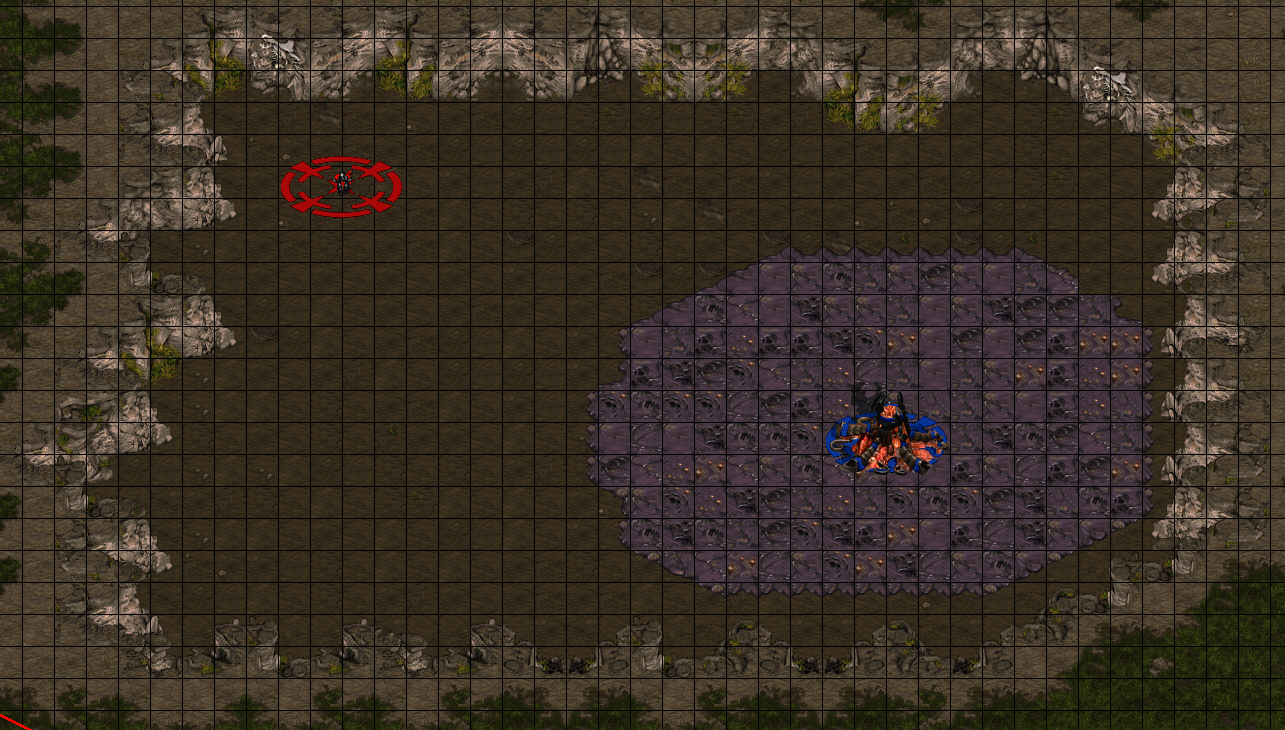
\includegraphics[width=0.9\textwidth]{ch4/nav_task}
    \caption{Example of map instance of the navigation task.}
    \label{fig:nav_task}
\end{figure}

We came up with this task by looking at the simplest problem human players have
to solve when playing StarCraft: moving units around the map.

The first sub-problem consisted in checking whether we could learn simple
policies based on location goals. We constructed 20 small maps in which a unit
was spawned on the opposite edge of map from the goal and had to reach the map
in the smallest amount of time. The agent received a reward of -1 for going
further away from the goal and 0 for getting closer to the goal. Reaching the
goal would give 10 of reward and would terminate the trial. You can see some of
those maps in Figure \ref{fig:nav_task}. We disabled \texttt{moveScreen*}
actions for both agents as we made the map small enough for all the relevant
information to be available. The Q-learning agent had access to the controlled
unit position and the goal position. Instead of using pixel-positions, we split
the plane in a 25 by 25 grid and provided all positions with respect to the
new grid. 

\subsection{Guided Navigation Task}

\begin{figure}[h]
    \centering
    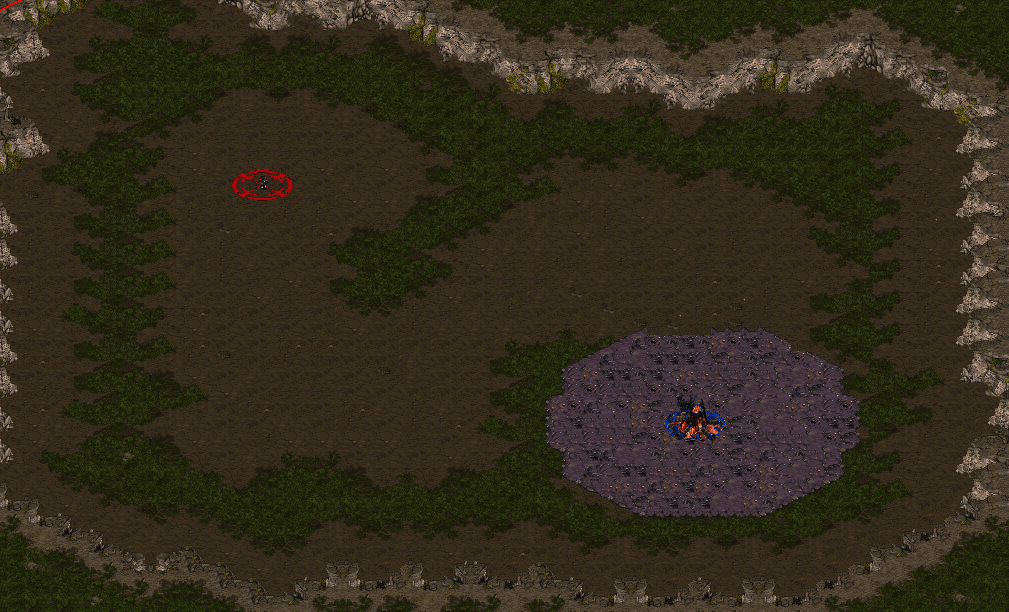
\includegraphics[width=0.9\textwidth]{ch4/guid_task}
    \caption{Example of map instance of the guided navigation task.}
    \label{fig:guid_task}
\end{figure}

The second task was a larger variation of the first one in which we also added
``death-zones''. Those zones acted as a repellent for the agents, giving a
reward of -100 when touched and acting as terminal states. The Q-learning agent
was given only one particular map configuration and access to the goal position,
while DQN had 20 maps to learn how to avoid danger maps. To guide the agent
visually we added a thick red border in the direction of the goal and we
assigned a different terrain pattern to the danger-zones. This time the map was
too large to cover the screen, so we locked the window to keep the unit always
at its center. Figure \ref{fig:guid_task} shows an example of one of those maps.

\subsection{Survival Task}

\begin{figure}[h]
    \centering
    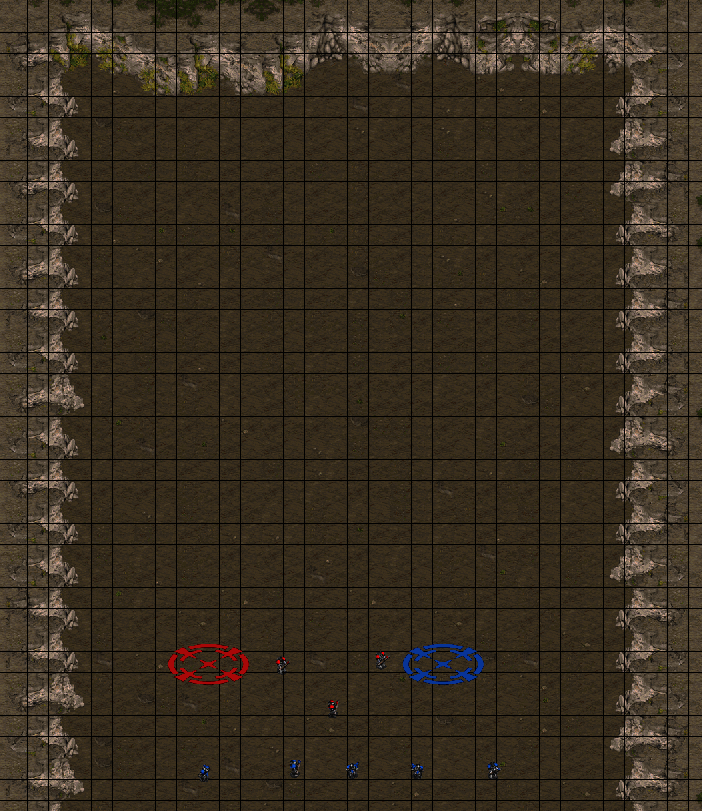
\includegraphics[width=0.5\textwidth]{ch4/surv_task}
    \caption{Example of map instance of the survival task.}
    \label{fig:surv_task}
\end{figure}

Our final task consisted in an interactive navigation problem. In particular,
one or more units was spawned in one of 20 maps in which all the allied units
were either close to aggressive enemy units or partly surrounded by them.
The agent would receive a reward of -10 if any of the units was killed, killing
a unit would account for a reward of 5, and 0 for any other event (or lack
thereof). Because of the multi-dimensionality of the space, it became possible
to receive different rewards at each time, so rewards received at some step $t$
were summed together before being sent to the agent. Figure \ref{fig:surv_task}
shows an example of one of those maps.


\section{RL Algorithms}

At the start of the project we decided that by the end of it we would have two
categories of testing algorithms: a classic model-free RL algorithm to test an
MDP-like setting and the newer DQN, a deep reinforcement learning algorithm, to
test learning policies purely from the visual input.

\subsection{Q-learning}

The choice of Q-learning as the test model-free algorithm was relatively
straightforward: Q-learning \citep{watkins1992q} is one of the most popular and
powerful model-free RL algorithms and it represents the foundation of many other
reinforcement learning algorithms. Given a standard MDP in the form of a tuple
$(S, A, T, R)$ where $S$ is the state space, $A$ is the action space, $T(s, s')$
is the transition probability distribution of moving from state $s$ to state
$s'$, and $R$ is the immediate reward received when moving from state $s$ to
state $s'$, Q-learning allows to iteratively find a policy that maximises the
expected total reward in a trial by learning from experience gained by using
some explorative policy (as opposed to on-policy reinforcement learning where
the policy used to gain ``experience'' is the same as the one that is being
learnt).

In particular, our algorithms works by updating an action-value function $Q(s,
a)$ using an $\epsilon$-greedy policy to gain new samples. Given a learning rate
$\alpha$ and a discount factor $\gamma$,

\begin{equation}
  Q(s_t, a_t) \leftarrow Q(s_t, a_t) +
  \alpha \left[ r_{t+1} + \gamma \max_a Q(s_{t+1}, a) - Q(s_t, a_t) \right].
\label{eq:ql}
\end{equation}

The agent policy in the evaluation phase then becomes

\begin{equation}
  \pi(s, a) = \operatornamewithlimits{argmax}_a Q(s, a).
\label{eq:ql2}
\end{equation}

It has been proved that this policy converges to the optimal policy $\pi^*$ given
enough samples from all state-action pairs
\citep{Sutton:1998:IRL:551283}. % TODO how?

The Q function can be represented as a table of values (a simple array) or can
be approximated using a function approximator, however a lot of literature has
highlighted difficulties in making Q-learning (and other model-free RL
algorithms) converge when the action-value function is approximated
\citep{sutton1999policy}. In some cases researchers managed to converge the
algorithms, but obtained significantly degraded policies
\citep{bertsekas2011approximate, baxter1999direct}.

\subsubsection{Task dependent state representation}

Providing a state representation for quickly testing the whole system ended up
resulting in a far more challenging problem than initially estimated. To be able
to extensively test the symbolic game state data being sent by the client we
wanted to obtain a useful state representation without having to use a black-box
function approximator such as an artificial neural network, as it would have
made it very hard to do automatic testings. Moreover we wanted to check and
explore how difficult it would have been to use standard RL techniques on
StarCraft's large state space.

\begin{sflisting}[caption=Example of a game state Lua table recorded by the
  agent, label=ls:sample] [standard]
{
  has_image = true,
  is_terminal = false,
  last_reward = -1,
  timestamp = 1459390526287,
  units = {
    [0] = {
      hp = 4,
      id = 0,
      is_allied = true,
      pos = { 544, 1602 },
      type = 1
    },
    [3] = {
      hp = 40,
      id = 3,
      is_allied = false,
      pos = { 666, 1733 },
      type = 1
    },
    [5] = {
      hp = 4,
      id = 5,
      is_allied = false,
      pos = { 612, 1722 },
      type = 1
    }
  }
}

\end{sflisting}

Listing \ref{ls:sample} shows a sample of the game state data in our
domain. We can see that it is difficult to represent such a representation in an
array because the data increases with the number of units. To create a
representation that we can use in a tabular fashion we must at least manually
compress the state in some way.

\begin{figure}[h]
    \centering
    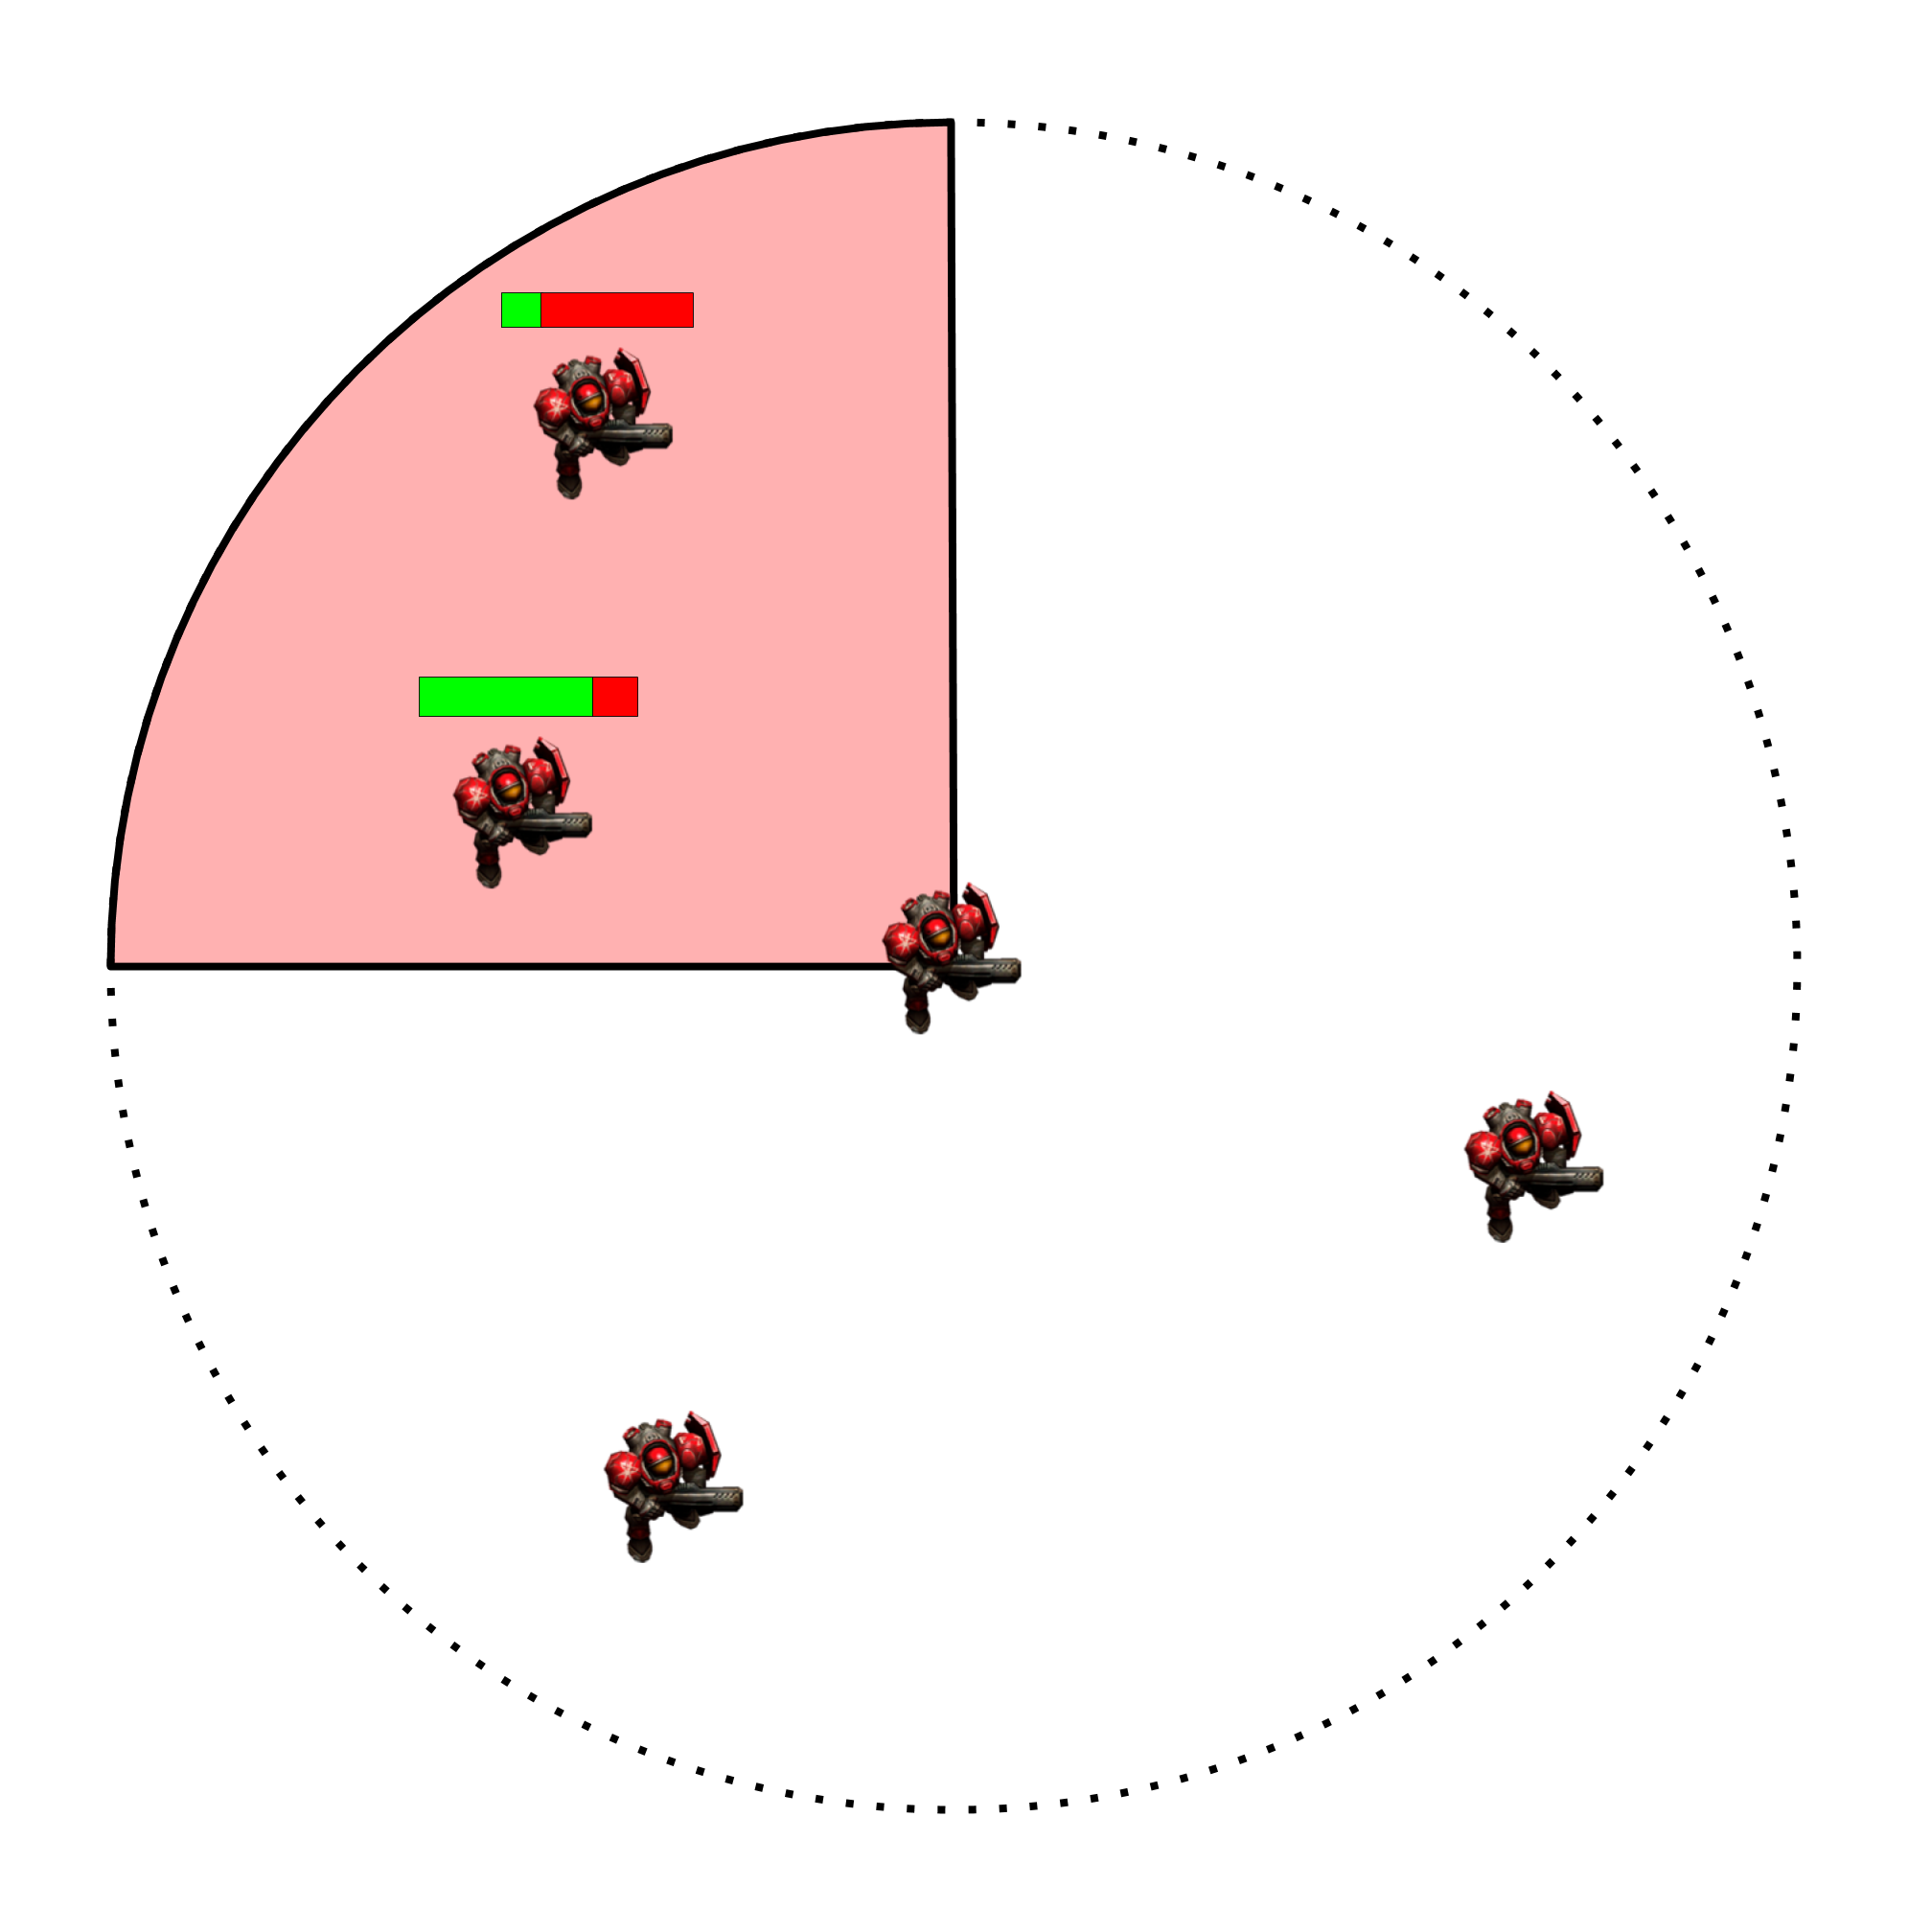
\includegraphics[width=0.6\textwidth]{ch4/discrete_state}
    \caption{Discretisation of state based on units health points.}
    \label{fig:discrete_state}
\end{figure}

We chose to approximate the state by discretise a potential function
\citep{thrun2005probabilistic} based on the health points of in-game units
relative to a particular selected allied unit (Figure \ref{fig:discrete_state}).
This was achieved by taking a particular unit as reference, filtering out
everything lying outside of the visible pixel radius, splitting then the
obtained space into a variable amount of slices. The value of each slice was
then calculated by obtaining the sum of all health ``value'' assigned to each
unit within a space. Given slice $p$ and $U_p$ units, the slice value $SV(p)$ is
computed as

\begin{equation}
  \begin{aligned}
    SV(p, \beta) = & 
    \begin{cases}
      \sum_{u \in U_p}{UV(u)} & \text{if } \sum_{u \in U_p}{UV(u)} < \beta \\
      \beta & otherwise\\
    \end{cases}, \\ \text{where } 
    UH(u) = &
    \begin{cases}
      1 & \text{if } \text{health}_u < 50\%\\
      2 & otherwise \\
    \end{cases} 
  \end{aligned}
\end{equation}

We created a pair of partitions for each class of unit representing allied units
and enemy units, and added to the top the value of the reference unit health,
ending up with a relatively large tensor as our index for our action-value
function (Figure \ref{fig:array_state}).

\begin{figure}[h]
    \centering
    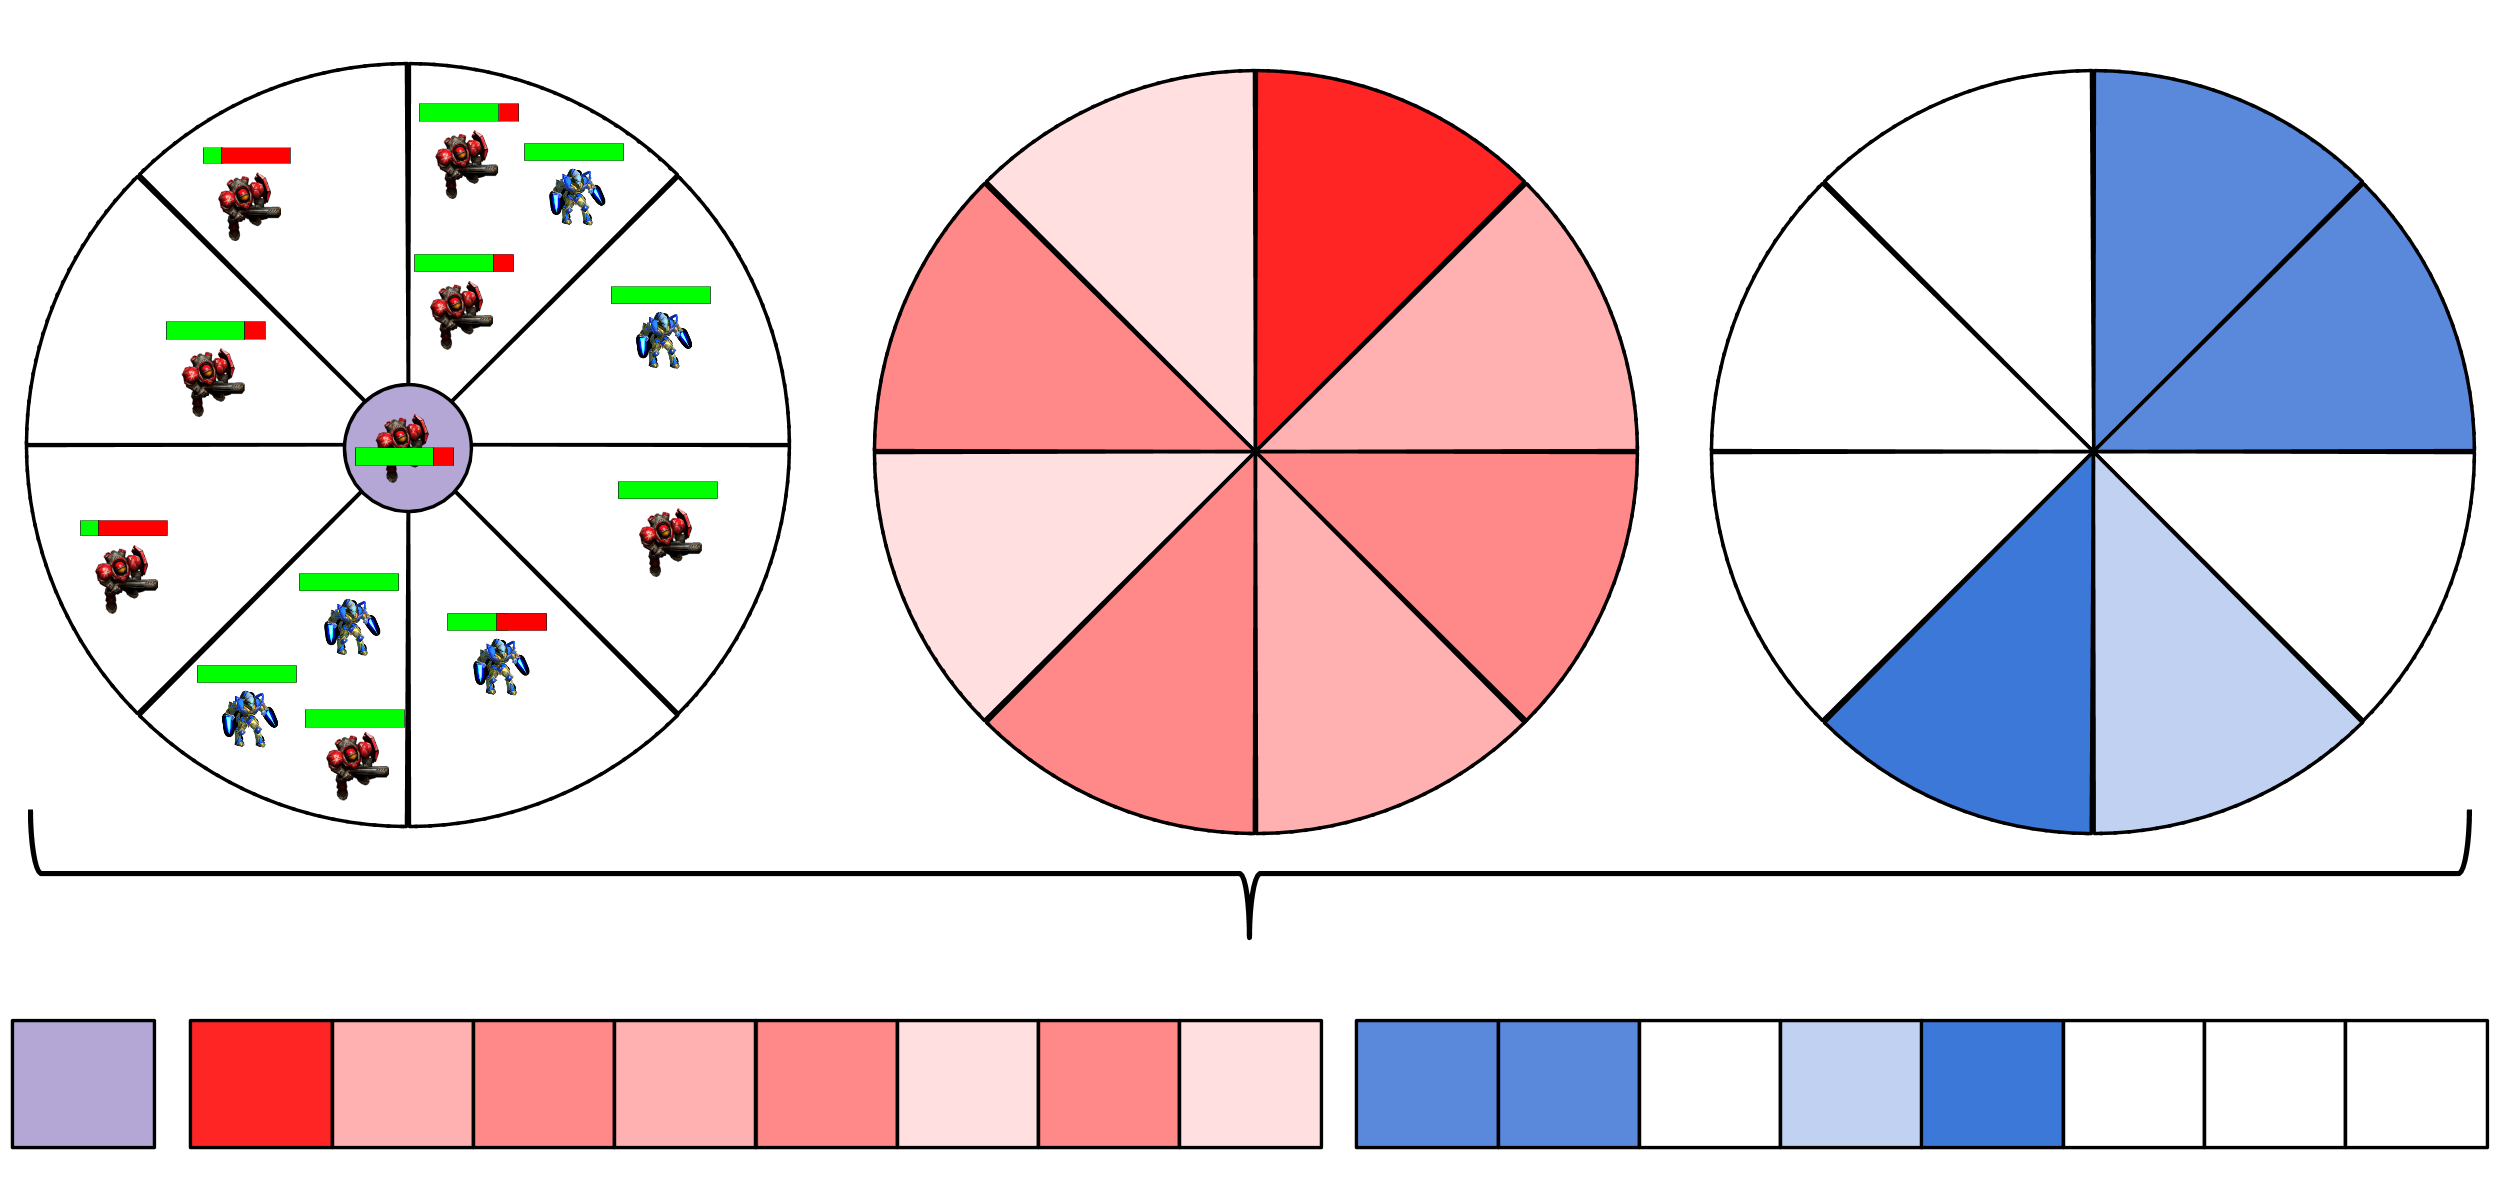
\includegraphics[width=\textwidth]{ch4/array_state}
    \caption{Mapping from slices to index tensor.}
    \label{fig:array_state}
\end{figure}

We could have also used a tile-coding technique\citep{sherstov2005function} to
stack multiple partitions of the same space (but different starting points) and
increase the generality of our state representation, but we didn't have the time
to finish its implementation.

This final technique is reasonable (as tests later confirmed) for our task, but
it wouldn't necessarily lend itself well to other scenarios. Our representation
for instance entirely lacks information about upgrades, bullets, visibility of
the map and state of the fog of war. It must be noted that with this
representation the problem becomes somewhat more complex than a standard MDP, as
we are not using the entirety of the available state information by filtering
everything outside of the image radius. We could have also used an observation
window to solve the partial observability problem, but we hypothesised that we
would obtain a good enough (but almost certainly suboptimal) policy in any case.

\subsection{Deep Q-learning}

The work described in this section is partially motivated by recent advances in
work that uses non-linear function approximators for reinforcement learning. The
\emph{Deep Q-Network} (DQN) algorithm \citep{mnih2013playing, mnih2015human} has
become one of the most popular variants of deep reinforcement learning, a
``new'' branch of reinforcement learning research that uses multi-layer ``deep''
neural networks (and other deep learning techniques) as functions approximators
to aid the decision-making process. They released their implementation together
with their Nature paper, both of which we used as a reference to develop a
version of DQN compatible with our interface.

DQN works by approximating the action-value function $Q(s, a)$ with a
Convolutional Neural Network. The network takes as input the state (in our case,
the screen image) and returns an array of values of the same size as the number
of available actions initialised when creating the network. The
$\epsilon$-greedy policy then chooses the action whose output value is highest,
or occasionally another random action.

\begin{figure}[h]
    \centering
    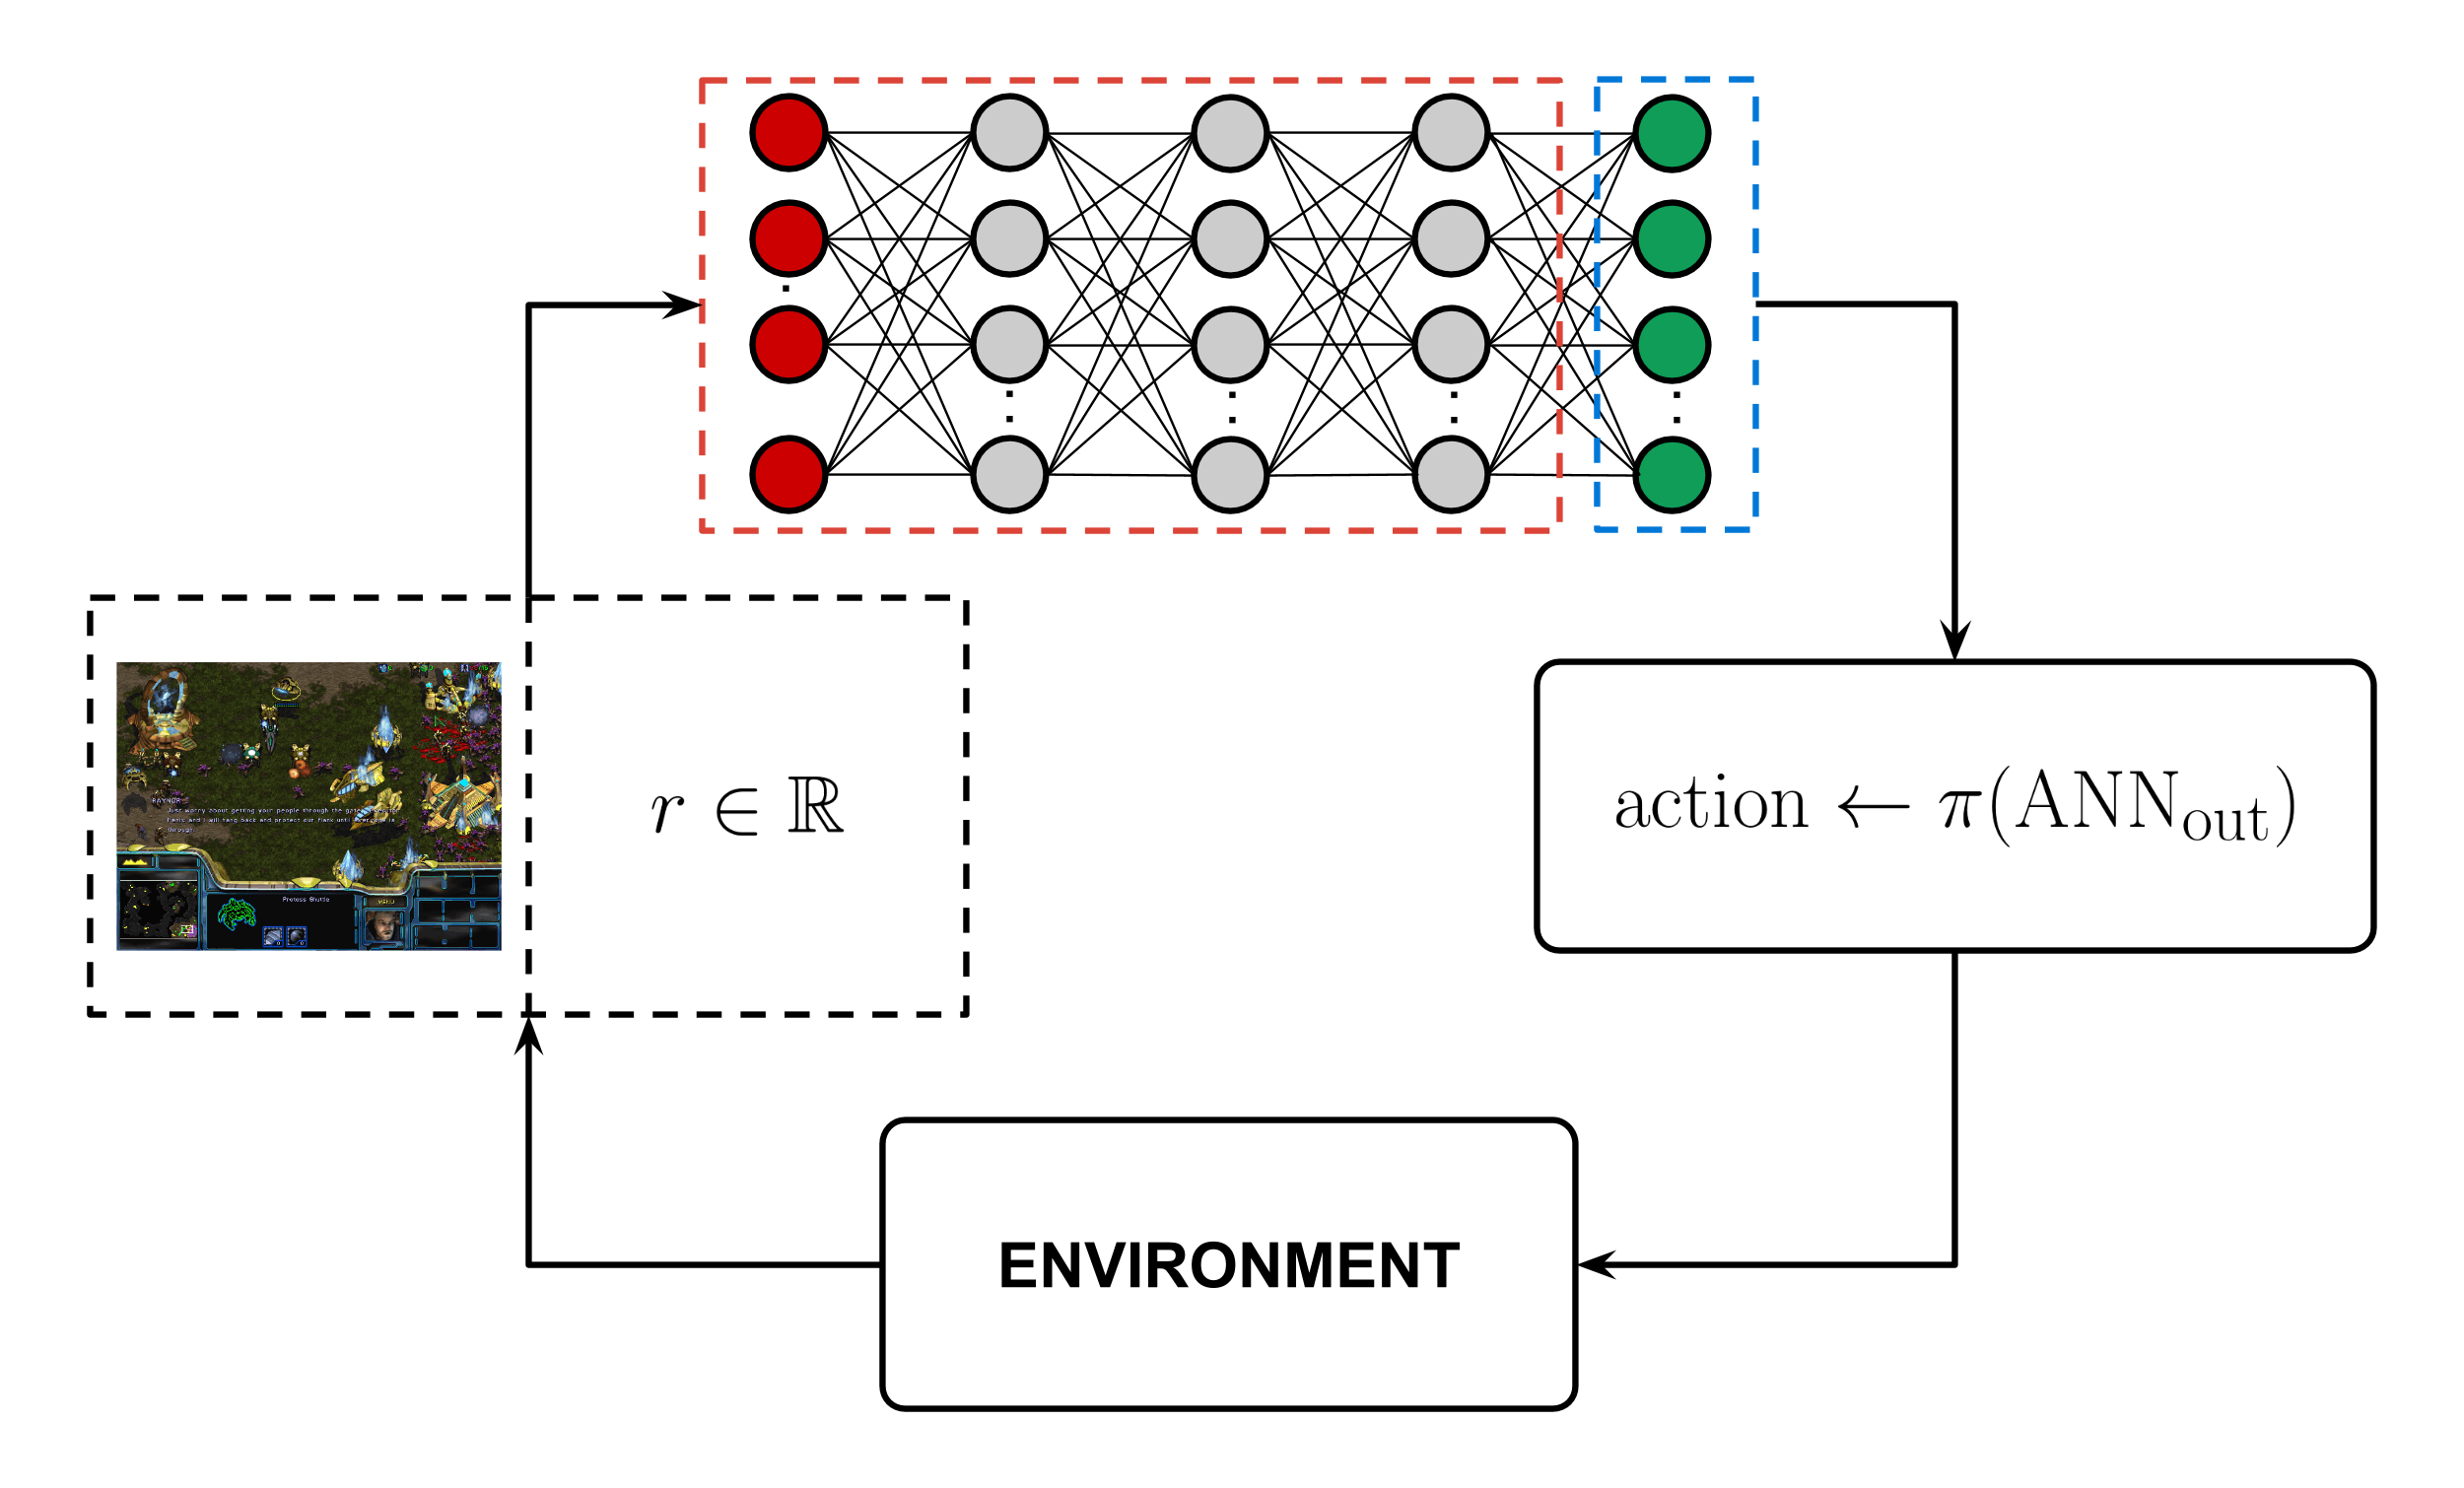
\includegraphics[width=\textwidth]{ch4/dqn}
    \caption{Deep Q-learning setting. The network outputs a value for each of
      the actions, which the policy can then use to select the preferred
      one to take.}
    \label{fig:dqn}
\end{figure}

If we consider the problem in a supervised learning fashion and imagine our
input dataset as just being generated by the interaction with the environment,
this setting then essentially becomes a regression problem with a neural
network trained using stochastic gradient descent algorithm that uses the
Q-learning update (Equation \ref{eq:ql}) as the loss function.

% TODO maybe put algorithm in here

Similarly to \cite{mnih2013playing}, our algorithms records all the tuples
containing the experience of the agent, keeps track of the newest ones using a
circular buffer, and samples from the buffer whenever the update step is called.
This functionality is called \textbf{Experience Replay} and removes the
correlation in the sequential observations, reducing the forgetting rate in the
network. To further reduce this correlation, the algorithm calculates the
temporal-difference error using a copy of the Q-network that is saved every now
and then. Finally in addition we added a maximum cap value to the
temporal-difference error to reduce big outliers and stop the weights from
changing too much when those appear.

\subsection{Multi-unit RL}

In the previous two sections we purposely avoided discussing an important design
problem related to our agent setting: by default they assume that the controlled
unit is one, while instead in StarCraft the player usually has to independently
control multiple units.

\begin{figure}[h]
    \centering
    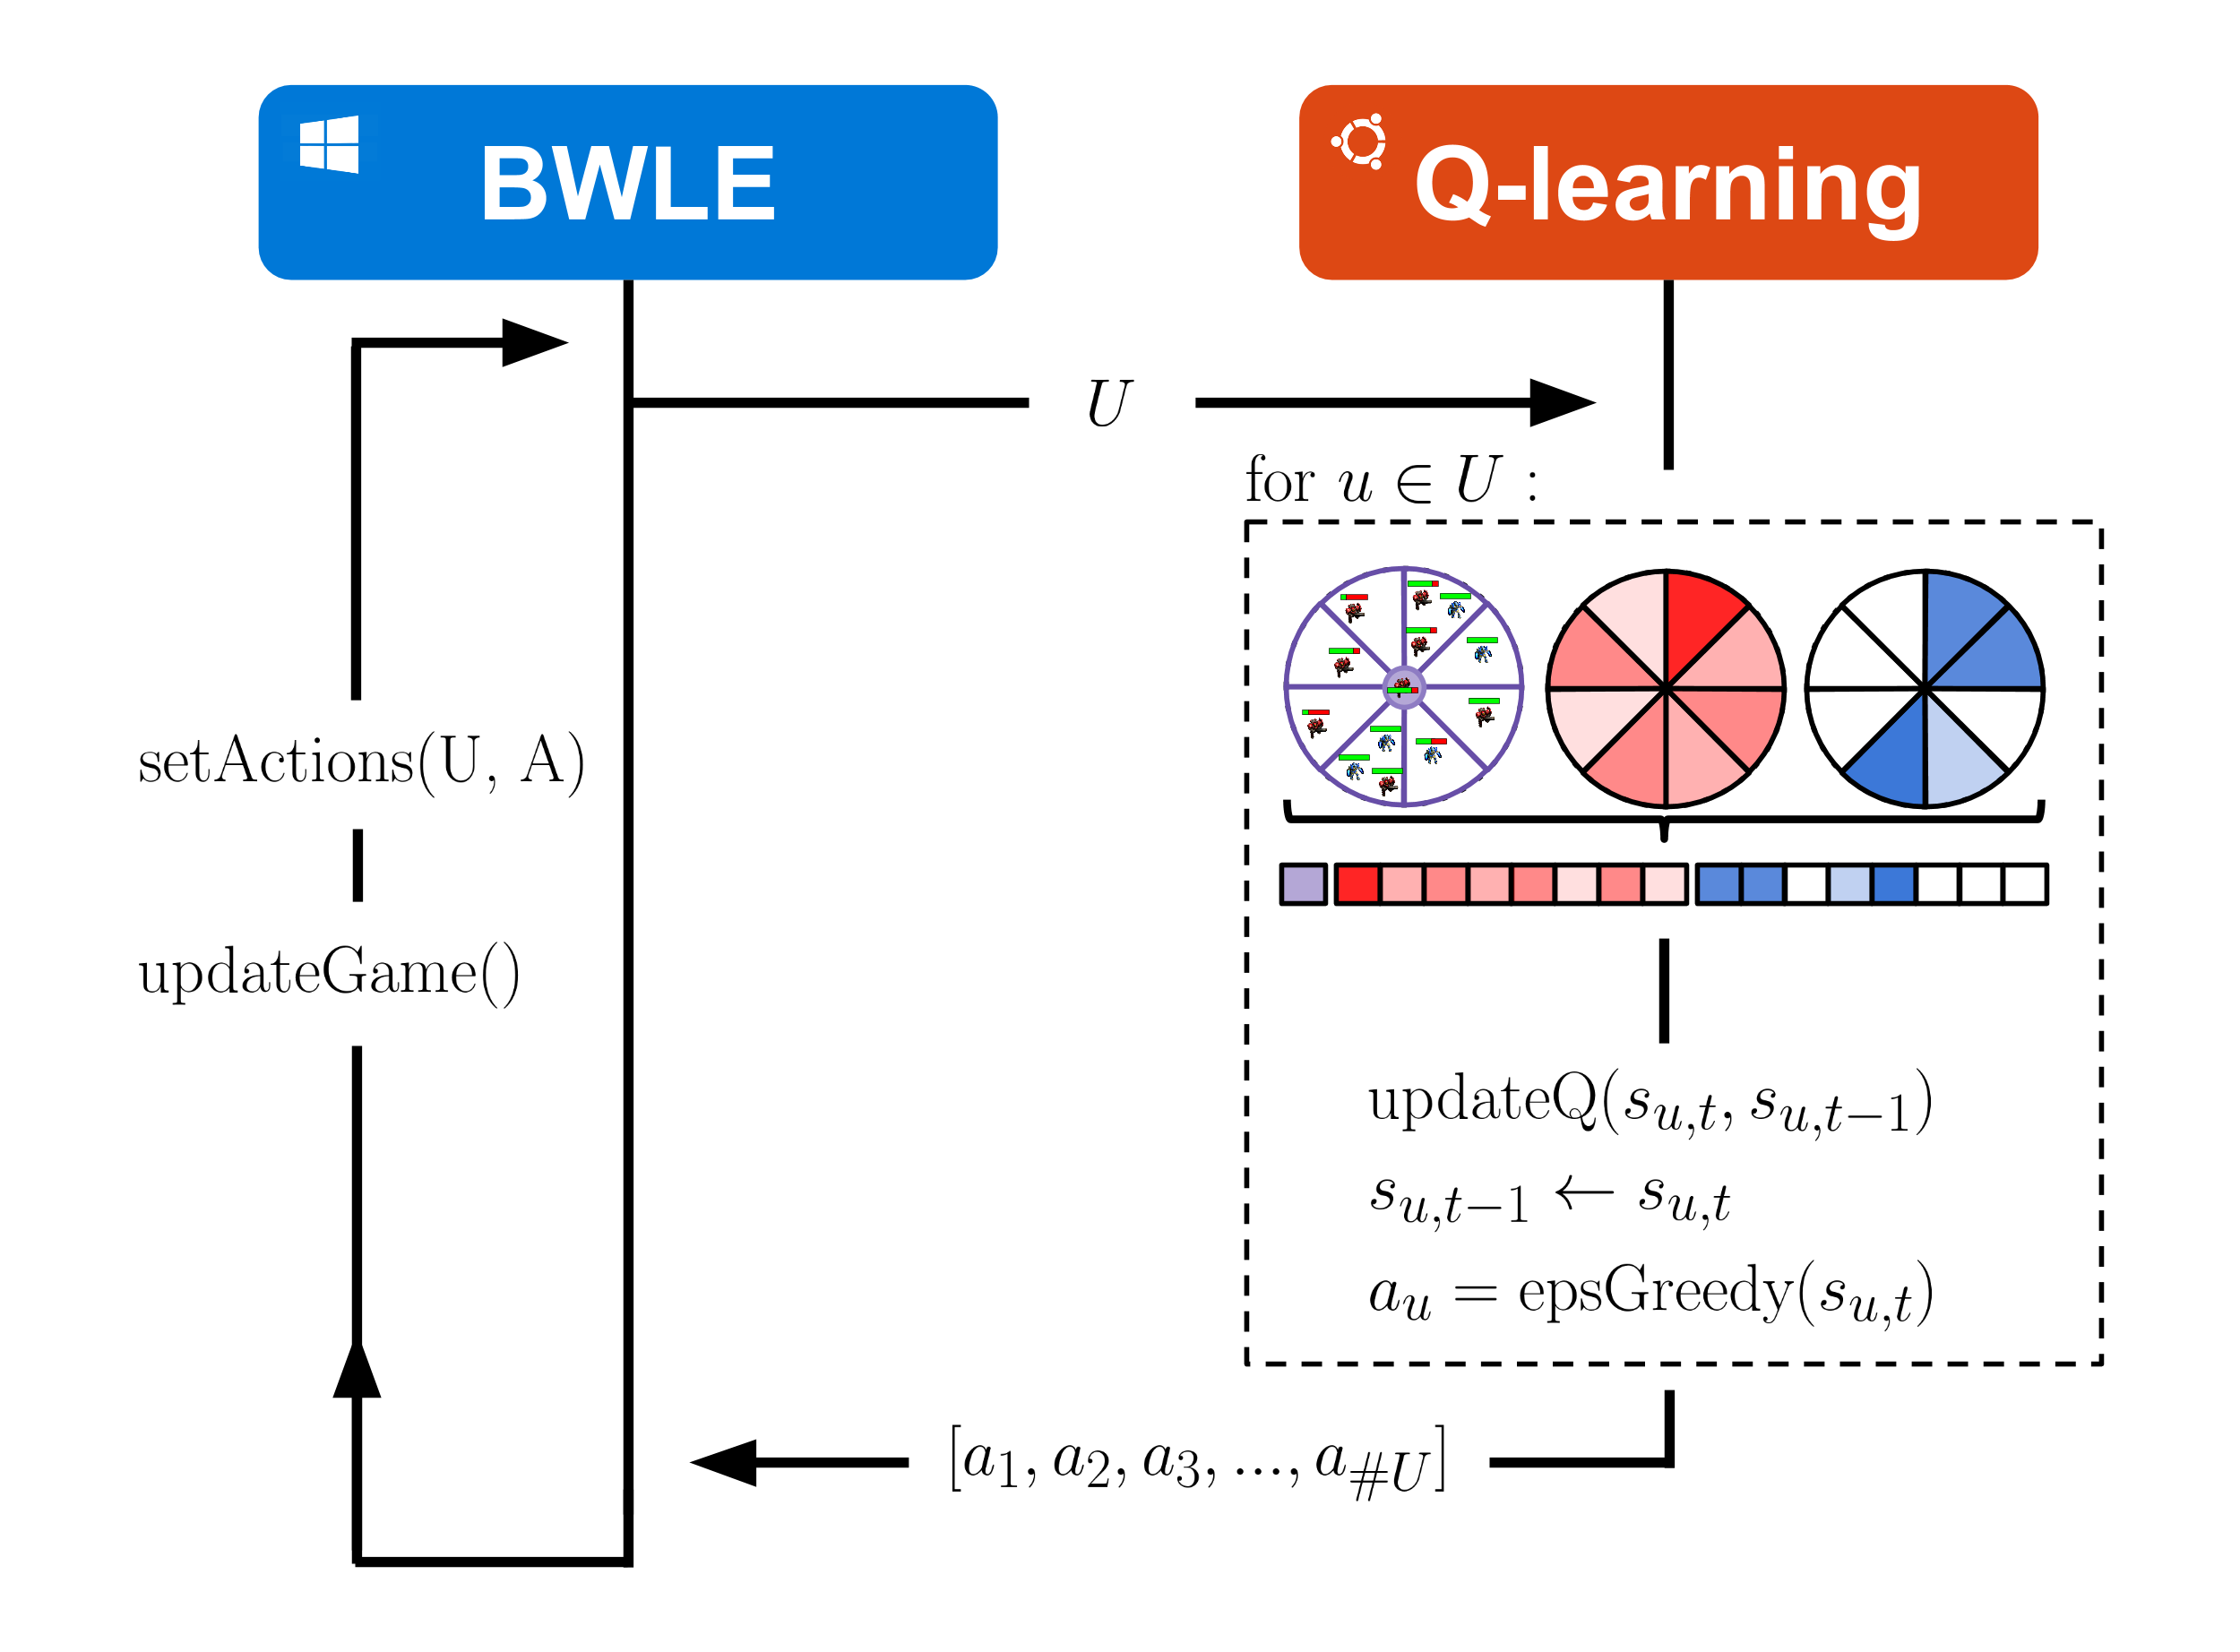
\includegraphics[width=0.9\textwidth]{ch4/parallelq}
    \caption{Visualisation of the parallel system for Q-learning.}
    \label{fig:parallelq}
\end{figure}

We didn't manage to find the time to review and implement multi-agent
reinforcement learning algorithms, so we decide to handle those multi-unit
scenarios in both Q-learning and Deep Q-learning by tweaking the
agent-environment settings.

The most effective way to coherently allow our algorithms to use multiple units
at the same time would have been to parametrise the actions by units ids, but
the actions space would then quickly explode. Additionally both our algorithms
(or at least their implementations) require the action number to be known a
priori. To avoid having to deal with the issue, we came up with a system to
optimise the execution of each unit action by parallelising the decision process
using the duration of the commanded primitive as a time buffer.

Q-learning was the easy to adapt, as the only required change to the algorithm
was to generate the state with respective to selected units and to parametrise
the action array by unit (Figure \ref{fig:parallelq}). Deep Q-learning was
harder to adapt because we had to take into account the visual window state. In
particular, to minimise the pixel variance we had to order the client to
position the window viewpoint on top of the unit to always keep it at the center
of the screen (Figure \ref{fig:paralleldqn}).

\begin{figure}[h]
    \centering
    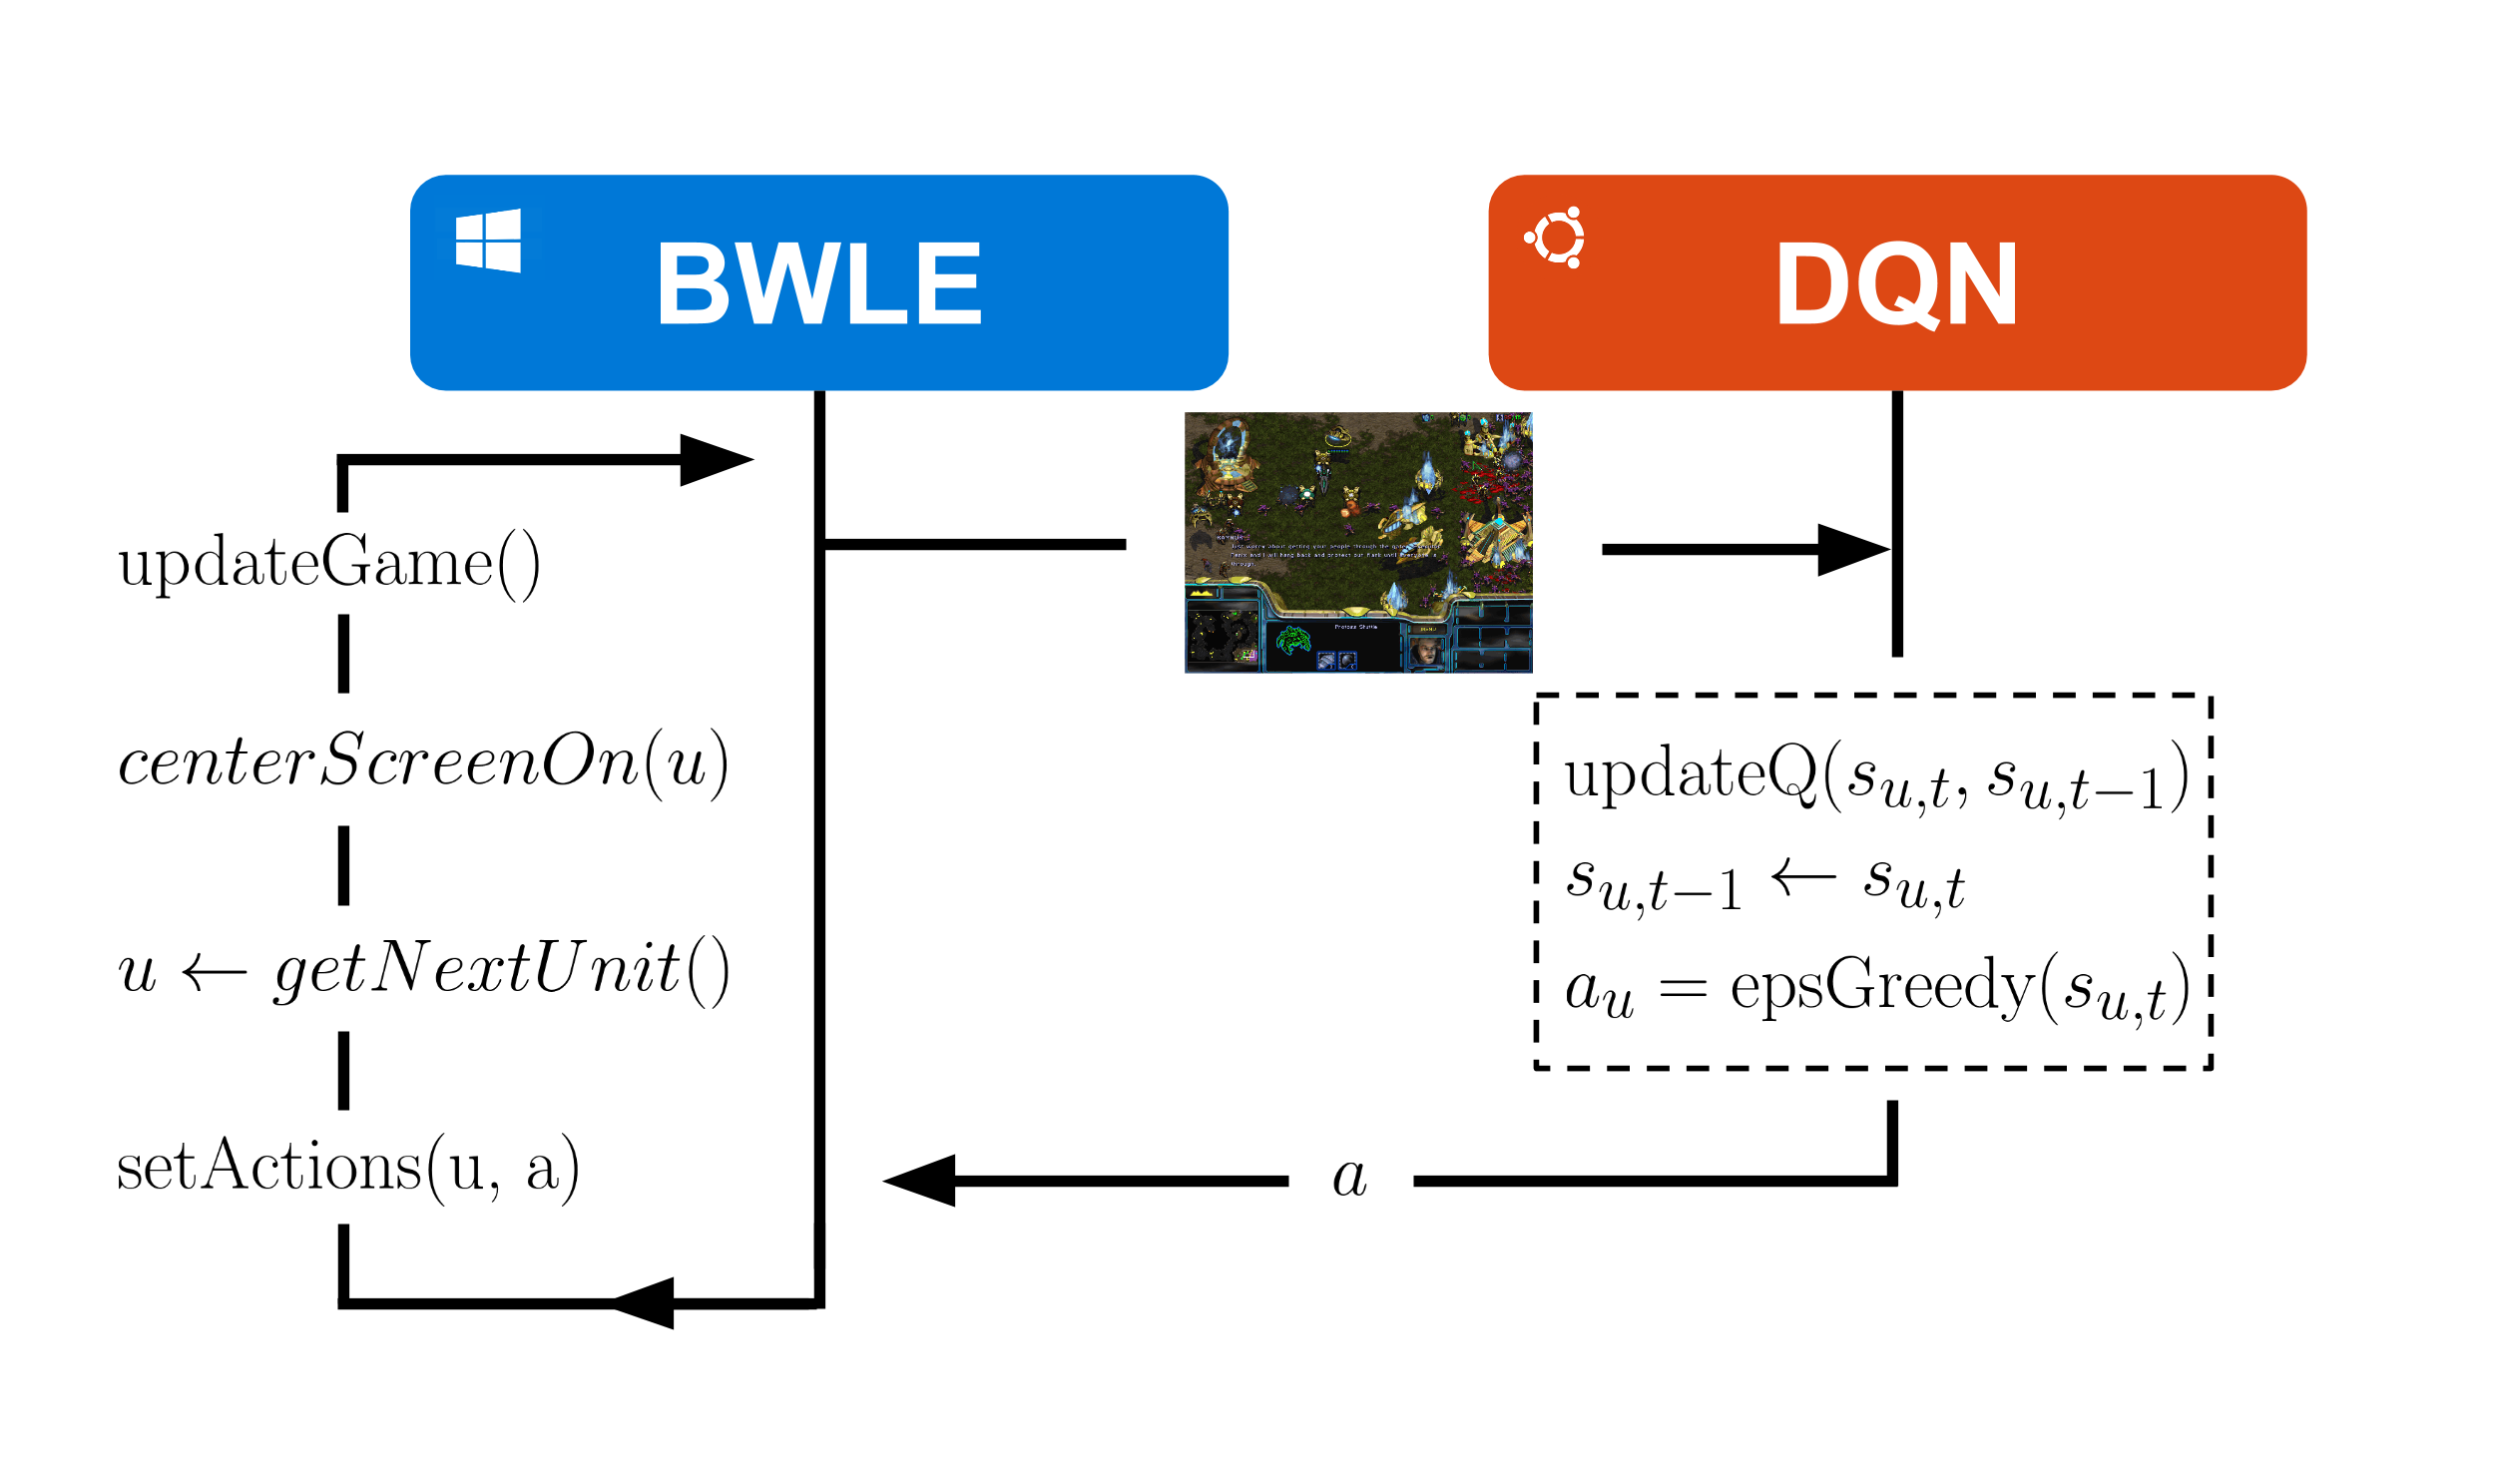
\includegraphics[width=0.9\textwidth]{ch4/paralleldqn}
    \caption{Visualisation of the parallel system for Deep Q-learning.}
    \label{fig:paralleldqn}
\end{figure}

This had the additional unexpected consequence of further randomising our
experiments, therefore allowing us to explore the state space much more quickly.
Unfortunately it also meant that the agent would not have any information about
the effect of its previous units' action choices over its future observations,
making the behaviour of allied units somewhat correlated with the agent policy.

% TODO maybe add that we had no way to check for this.

\section{Hardware Setup}

All our development was carried out on a Ubuntu workstation equipped with a
Intel i7-4790K CPU, 16GB of RAM, an NVIDIA GTX970, and 250GB of solid state
storage disk. Half of the cores and memory was assigned to a Windows 7 virtual
machine, making it possible to develop the entire pipeline on one machine. The
evaluation of the platform was done using the previously mentioned virtual
machine and a Dell Server equipped with a 64-cores Intel Xeon E5-2698 CPU (of
which we used only 8) and an NVIDIA GTX980Ti.
